% *******************************************************************************
% * Copyright (c) 2007 by Elexis
% * All rights reserved. This document and the accompanying materials
% * are made available under the terms of the Eclipse Public License v1.0
% * which accompanies this distribution, and is available at
% * http://www.eclipse.org/legal/epl-v10.html
% *
% * Contributors:
% *    G. Weirich
% *
% *  $Id: konzepte.tex 2936 2007-07-30 15:05:01Z rgw_ch $
% *******************************************************************************
% !Mode:: "TeX:UTF-8" (encoding info for WinEdt)

\section{Kontakte}
\label{kontakt}
In Elexis ist jede Person oder Firma, die in irgendeiner Beziehung zur Praxis
steht, zunächst mal ein \glqq Kontakt\grqq{}. Kontakte werden in der
Kontakt-Perspektive eingegeben oder geändert.
\begin{flushleft}
    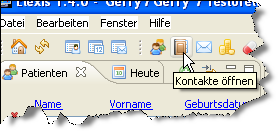
\includegraphics{images/contactperspective}
\end{flushleft}


Es gibt folgende Typen von Kontakten:
\begin{itemize}
  \item Person
	\begin{itemize}
  		\item Mandant
  		\item Anwender
  		\item Patient
  		\item Andere
    \end{itemize}
    \item{Organisation}
    \begin{itemize}
      \item{Labor}
      \item {Andere}
    \end{itemize}
\end{itemize}


\section{Anwender und Mandanten}
Jemand, der eine Rechnungsstelle (in der Schweiz z.B. eine eigene ZSR-Nummer) hat, ist ein \textit{Mandant}. Jeder Vorgang in Elexis (Konsultation, Labor, Rezept etc.) läuft immer unter Verantwortung und auf Rechnung genau eines Mandanten. \index{Mandant}

\medskip

Jemand, der das Programm bedienen darf, ist ein \textit{Anwender}. Ein Anwender arbeitet immer im Auftrag eines bestimmten Mandanten.

Zu jedem Zeitpunkt gibt es in Elexis also einen aktuellen Mandanten und einen aktuellen Anwender.
\index{Anwender}Mandant und Anwender können auch identisch sein (Wenn der
Mandant selbst am PC arbeitet).
Ein Anwender kann auch die Mandantenzuordnung ändern (Wenn eine MPA in einer Gruppenpraxis beispielsweise für unterschiedliche
Mandantinnen arbeitet).
\index{Gruppen}\index{Rechte}
Anwender haben bestimmte, individuell einstellbare Rechte, mit denen man sehr
fein steuern kann, wer welche Aktionen innerhalb von Elexis steuern kann.
Anwender können auch in Gruppen zusammengefasst sein, die bestimmte gemeinsame
Rechte definieren (z.B. Gruppen \glqq MPAs\grqq{} oder \glqq Ärzte\grqq{}). Eine
spezielle Gruppe ist die Gruppe \glqq Admin\grqq{}: Wer zu dieser Gruppe gehört,
hat automatisch \textit{alle} Rechte.
\textbf{Wichtig}: Auch wenn Ihnen das zunächst unlogisch erscheinen mag: Auch
der Chef sollte normalerweise nicht als Admin \index{Administrator} arbeiten.
Der Grund ist, dass der Admin-Account auch irreversible Löschungen und andere
sehr unangenehme Veränderungen erlaubt. Wie schnell hat man in der Hektik des
Alltags mal einen falschen Knopf geklickt!
Deswegen: Arbeiten Sie im Alltag mit einem Account, der genau diejenigen Rechte
hat, die Sie auch im Alltag brauchen. Erstellen Sie für sich einen zweiten
Account, welcher der Gruppe Admin zugeordnet ist, und melden Sie sich nur dann
unter diesem Account an, wenn es wirklich notwendig ist.

Das Konzept der Gruppen und Rechte ist ab Seite \pageref{sec:gruppen} ff.
genauer erklärt.

\section{Konsultationen, Fälle, Garanten und Kostenträger}
\index{Konsultation}\index{Fall}\index{Garant}\index{Krankenkasse}\index{Kostenträger}
\index{Leistungserbringer}\index{Abrechnung}Jeder in Elexis festgehaltene Kontakt zwischen Praxispersonal und Patient ist eine \textit{Konsultation}. Wenn die Konsultation verrechnet wird, dann geht die Verrechnung zugunsten desjenigen Mandanten, für welchen der eingeloggte Anwender tätig war.

Jede Konsultation ist auch einem \textit{Fall} zugeordnet. Ein Fall ist hier eher eine versicherungstechnische, als eine medizinische Einheit: Der Fall sammelt alle Konsultationen, welche mit demselben Abrechnungssystem (s. \ref{settings:abrechnungssystem} auf S. \pageref{settings:abrechnungssystem}) abgerechnet werden. Dies kann manchmal identisch mit dem medizinischen Fallbegriff sein (Ein Unfall, welcher über einen bestimmten Versicherer mit einer bestimmten Fallnummer abgerechnet wird), oder er kann auch keinen Zusammenhang mit einem medizinischen Fall haben (z.B. wird in der Schweiz im Allgemeinen ein allgemeiner Fall \glqq Krankheit\grqq{} erstellt werden, der alle KVG-Konsultationen sammelt.

Ein Fall kann immer nur einen Patienten und ein Abrechnungssystem haben, kann aber durchaus  Konsultationen mehrerer Mandanten beinhalten. (Es wird dann für jeden Mandanten eine separate Rechnung erstellt).

\clearpage

\section{Leistungsabrechnung}
\index{Leistungscodes}\index{abrechnen}
\begin{wrapfigure}{l}{7.5cm}
    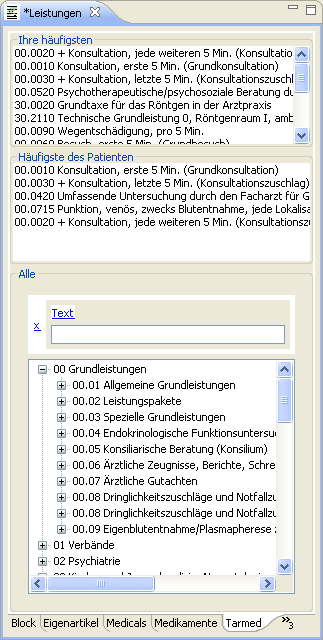
\includegraphics[width=7.5cm]{images/leistungen1}
    \caption{Leistungen}
    \label{fig:leistungen}
\end{wrapfigure}
Die Leistungscodes, die verrechnet werden können, werden einerseits von Plugins beigesteuert (z.B. Elexis-Arzttarife-Schweiz), andererseits durch von Ihnen selbst definierte Leistungsblöcke (s. weiter unten).

Alle im System vorhandenen Leistungscodesysteme sind im Fenster \glqq Leistungen\grqq{} (Abb. \ref{fig:leistungen}) untergebracht: Am unteren Rand des Fensters sehen Sie für jedes installierte Leistungscodesystem einen Reiter.

Dieses Fenster erscheint jeweils dann, wenn Sie vom Konsultationsfenster aus \glqq{}Verrechnung\grqq{} anklicken. Der Aufbau ist für jedes Leistungscodesystem gleich:

Im obersten Teilfenster stehen die von Ihnen am häufigsten angewendeten Codes dieses Leistungssystems, sind dadurch also im raschen Zugriff ohne suchen. Die Liste wird laufend aktualisiert, und je häufiger Sie einen bestimmten Code verwenden, desto weiter oben erscheint er beim nächsten Öffnen des Fensters.

\medskip
Im mittleren Teil erscheinen die bei diesem Patienten bisher am häufigsten verwendeten Codes, welche nach demselben Prinzip sortiert sind. Im untersten Teilfenster schliesslich steht das gesamte Leistungscodesystem in der vorgegebenen Systematik zur Verfügung.

\bigskip

Um einen Code zu verrechnen, können Sie ihn  aus irgendeinem der drei Abschnitte ins Verrechnung-Fenster ziehen, oder auch per Doppelklick anwählen. Manche Plugins können auch einen \glqq Optifier\grqq (Optimizer/Verifier) beinhalten, welcher Fehler erkennt bzw. Korrekturen anbringen kann. So wird etwa das Tarmed-Plugin einerseits z.B. die doppelte Verrechnung des Codes \textit{00.0010 Konsultation erste 5 Minuten} mit einer Fehlermeldung verweigern (Verifier), und andererseits wird es, wenn Sie den Code \textit{00.0030 Konsultation letzte 5 Minuten} abrechnen, automatisch auch den Code 00. 0010 dazunehmen, da 00.0030 ja immer mit 00.0010 kombiniert wird (Optimizer).
Bei \textit{Artikeln}, welche bei Direktabgabe auch von diesem Fenster aus verrechnet werden können, wird bei Verrechnung jeweils automatisch auch der Lagerbestand entsprechend nachgeführt.

\subsection{Leistungsblöcke und Eigenleistungen}
Als weitere Arbeitserleichterung erlaubt Elexis auch, mehrere Leistungscodes, auch aus ganz unterschiedlichen Codesystemen, zu Blöcken zusammenzufassen, die dann komplett oder teilweise verrechnet werden können. Solche Blöcke können nebst vordefinierten Leistungscodes aller installierten Codesysteme auch selbstdefinierte Elemente enthalten.

\section{Artikel und Lager}
\index{Artikel}\index{Medikament}\index{Lager}
 Alles was eingekauft, gelagert, abgegeben oder rezeptiert werden kann, ist ein \textit{Artikel}.
 Artikel sind in Klassen organisiert, beispielsweise \textit{Medikament},
 oder \textit{MiGeL} oder \textit{Büromaterial}.
 Elexis kann jeden Artikel, den es kennt, als \textit{Lagerartikel} aufnehmen.

 Ein Lagerartikel ist ein Artikel, dessen Bestand monitorisiert wird, und der bei Bedarf auch halbautomatisch nachbestellt werden kann.
 Weitere Informationen zu Artikeln und Lager finden Sie bei der Beschreibung der entsprechenden View (S. \pageref{view:artikel} ff.)

 \section{Mehrere Instanzen gleichzeitig}
 \index{gleichzeitig}
 Sie können Elexis problemlos mehrfach starten und dann in verschiedenen
 Fenstern unterschiedliche Perspektiven oder verschiedene Patienten anzeigen.
 Einzelne Elemente können auch mit Cut\&Paste zwischen den laufenden Instanzen
 ausgetauscht werden.
 Anwendungsbeispiele:
 \begin{itemize}
   \item Sie arbeiten an einem Patienteneintrag und es kommt ein Telefon
   betreffend eines anderen Patienten. Anstatt Ihre Arbeit zu verlassen, bringen
   Sie die zweite Elexis-Instanz in den Vordergrund und suchen dort den neuen
   Patienten auf.
   \item Die MPA möchte an ihrem Arbeitsplatz Agenda und Patientendaten
   gleichzeitig im Blick haben. Spendieren Sie ihr einen zweiten Monitor (statt
   eines zweiten PC's), schliessen Sie beide Monitore an einer DualHead-fähigen
   Grafikkarte am selben PC an und schieben Sie in jeden Monitor eine eigene
   Instanz von Elexis.
   \item Während Elexis mit einem langwierigen Rechnungsdruck beschäftigt ist,
   möch\-ten Sie nicht untätig herumsitzen. Kein Problem, starten Sie eine zweite
   Instanz von Elexis und arbeiten Sie dort weiter. (Sie könnten natürlich auch
   einen Kaffee trinken oder einen Spaziergang machen).
   \item Sie erstellen einen Brief, möchten aber einzelne Stellen aus einem
   anderen Brief herüberkopieren. Laden Sie in der einen Elexis-Instanz den
   alten Brief, erstellen Sie in der anderen den neuen Brief und kopieren Sie
   das gewünschte mit Cut\&Paste.
 \end{itemize}

\section{Plugins}
Dieses Konzept wird auf Seite \pageref{expl:plugins} genauer besprochen. Hier nur soviel: Elexis ist nach allen Seiten frei erweiterbar. Es gibt nicht nur eine vorgegebene Zahl von \glqq Modulen\grqq{}, sondern tatsächlich können jederzeit auch von Dritten neue Funktionen programmiert werden, von denen zum Zeitpunkt des Programmreleases noch gar nichts bekannt war. Dies geschieht in Form von sogenannten \glqq Plugins\grqq{}. Plugins können beispielsweise für Statistik, Buchhaltung, Import von Labordaten, Anbindung von Apparaten, Export von KG-Daten, neue Abrechnungssysteme, neue Diagnosesysteme usw. programmiert werden.

Ein Elexis-Plugin ist also einfach ein Programm mit im Prinzip beliebigen Fähigkeiten, welches die Eigenschaft hat, mit Elexis zusammenarbeiten zu können.

Es kann weder in diesem Handbuch noch sonstwo eine abschliessende Aufzählung aller Plugins geben, weil niemand wissen kann, welche Plugins von unabhängigen Anwendern bei unabhängigen Programmierern in Auftrag gegeben worden sind. 